\documentclass[final]{beamer}
\mode<presentation>{\usetheme{default}}

\usepackage[T1]{fontenc}
\usepackage[utf8]{inputenc}
\usepackage{lmodern}
\usepackage[orientation=landscape,size=a1,scale=1.08]{beamerposter}
\usepackage{graphicx}
\usepackage{booktabs}
\usepackage{array}
\usepackage{amsmath}
\usepackage[table]{xcolor}
\usepackage{colortbl}
\usepackage{tikz}
\usepackage{pgfplots}
\pgfplotsset{compat=1.18}
\usetikzlibrary{positioning}

\definecolor{ucblue}{HTML}{0039A6}
\definecolor{ucdark}{HTML}{001A4D}
\definecolor{ucgold}{HTML}{C99700}
\definecolor{uclight}{HTML}{EEF3FF}

\setbeamertemplate{navigation symbols}{}
\setbeamercolor{background canvas}{bg=white}
\setbeamercolor{title in headline}{fg=white,bg=ucblue}
\setbeamercolor{author in headline}{fg=white,bg=ucgold}
\setbeamercolor{block title}{fg=white,bg=ucblue}
\setbeamercolor{block body}{fg=black,bg=white}
\setbeamercolor{alertblock title}{fg=white,bg=ucdark}
\setbeamercolor{alertblock body}{fg=black,bg=uclight}
\setbeamercolor{exampleblock title}{fg=white,bg=ucgold}
\setbeamercolor{exampleblock body}{fg=black,bg=uclight}

\setbeamerfont{title}{size=\LARGE,series=\bfseries}
\setbeamerfont{author}{size=\large}
\setbeamerfont{institute}{size=\normalsize}
\setbeamerfont{block title}{size=\large,series=\bfseries}
\setbeamerfont{block body}{size=\normalsize}

\newlength{\sepwidth}
\newlength{\colwidth}
\setlength{\sepwidth}{0.025\paperwidth}
\setlength{\colwidth}{0.30\paperwidth}
\newcommand{\separatorcolumn}{\begin{column}{\sepwidth}\end{column}}

\title{Continuacion Automatica de Playlists (APC)}
\author{Agustin Llambias \and Amaya Quero \and Larry Uribe}
\institute{Pontificia Universidad Catolica de Chile -- IIC3633 Sistemas Recomendadores (2026-1)}

\begin{document}
\begin{frame}[t]

\begin{beamercolorbox}[wd=\textwidth,ht=6.2cm,dp=0.8cm,leftskip=1.3cm,rightskip=1.3cm]{title in headline}
  {\usebeamerfont{title}\inserttitle\par}
  \vspace{0.35cm}
  {\large \textbf{Two-Stage Hybrid vs. Baselines Secuenciales y Colaborativos}\par}
  {\usebeamerfont{author}\insertauthor\par}
  {\usebeamerfont{institute}\insertinstitute}
\end{beamercolorbox}
\begin{beamercolorbox}[wd=\textwidth,ht=0.28cm,dp=0cm]{author in headline}\end{beamercolorbox}
\vspace{0.6cm}

\begin{columns}[t]
\separatorcolumn

\begin{column}{\colwidth}
\begin{alertblock}{Pregunta de investigacion}
\textbf{Que tan competitivo es un sistema APC local y reproducible de dos etapas frente a metodos mas fuertes, al evaluar ranking y metricas beyond-accuracy?}
\end{alertblock}

\begin{block}{Datos y protocolo experimental}
\begin{itemize}
  \item Spotify Playlists (Kaggle), muestra deterministica por hash.
  \item Corrida principal: 30\% (63,851 playlists evaluadas).
  \item Corrida de sensibilidad: 20\%.
  \item Evaluacion: \textit{leave-last-out}, minimo 3 canciones por playlist.
\end{itemize}
\end{block}

\begin{block}{Metodologia propuesta}
\textbf{Two-Stage Hybrid}
\begin{enumerate}
  \item Retrieval por co-ocurrencia item-item (normalizacion coseno).
  \item Reranking hibrido con senales: cooc, popularidad, artista y nombre de playlist.
\end{enumerate}

\textbf{Comparadores}
\begin{itemize}
  \item Sequential Markov
  \item Collaborative ItemKNN
  \item Random, Most Popular, Playlist Name Popular
\end{itemize}
\end{block}

\begin{block}{Pipeline}
\centering
\begin{tikzpicture}[node distance=0.82cm,>=latex,scale=0.94,transform shape]
  \node[draw,rounded corners,fill=uclight,minimum width=3.5cm,minimum height=1.0cm] (c1) {Contexto};
  \node[draw,rounded corners,fill=uclight,right=1.2cm of c1,minimum width=3.4cm,minimum height=1.0cm] (c2) {Retrieval cooc};
  \node[draw,rounded corners,fill=uclight,right=1.2cm of c2,minimum width=3.6cm,minimum height=1.0cm] (c3) {Reranking};
  \node[draw,rounded corners,fill=ucgold!25,right=1.2cm of c3,minimum width=2.6cm,minimum height=1.0cm] (c4) {Top-10};
  \draw[->,thick,ucblue] (c1) -- (c2);
  \draw[->,thick,ucblue] (c2) -- (c3);
  \draw[->,thick,ucblue] (c3) -- (c4);
\end{tikzpicture}
\end{block}
\end{column}

\separatorcolumn

\begin{column}{\colwidth}
\begin{block}{Resultados principales (30\%)}
\centering
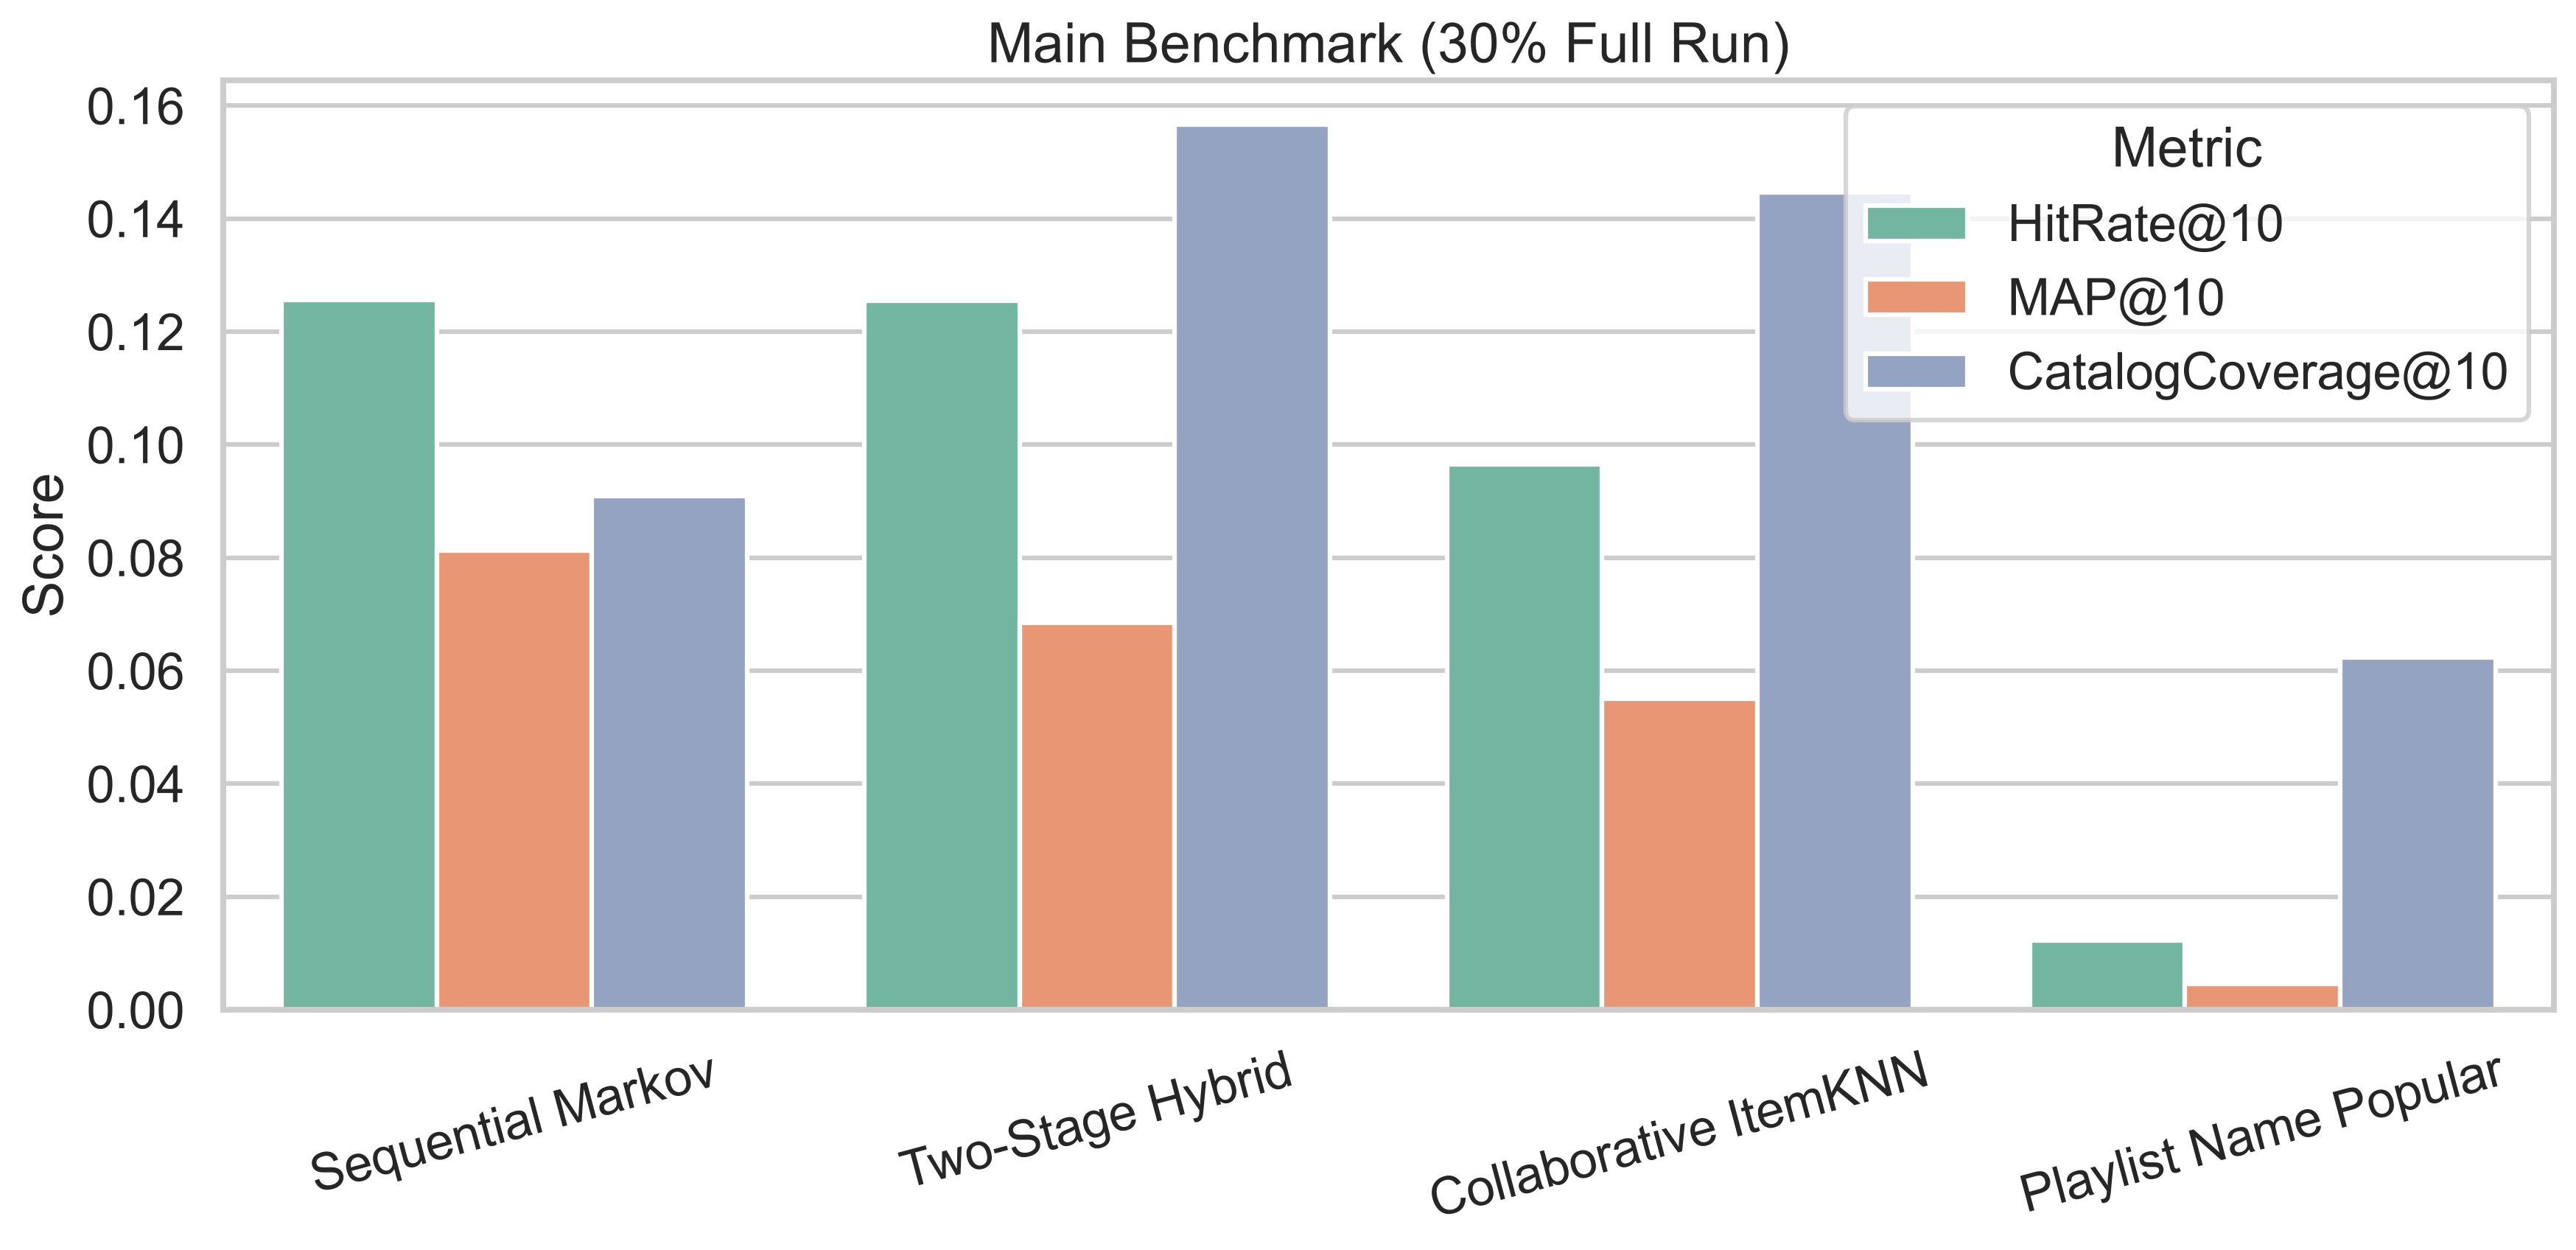
\includegraphics[width=0.98\linewidth]{figures/fig_main_benchmark.png}
\end{block}

\begin{columns}[t,totalwidth=\linewidth]
\begin{column}{0.49\linewidth}
\begin{block}{Ablations}
\centering
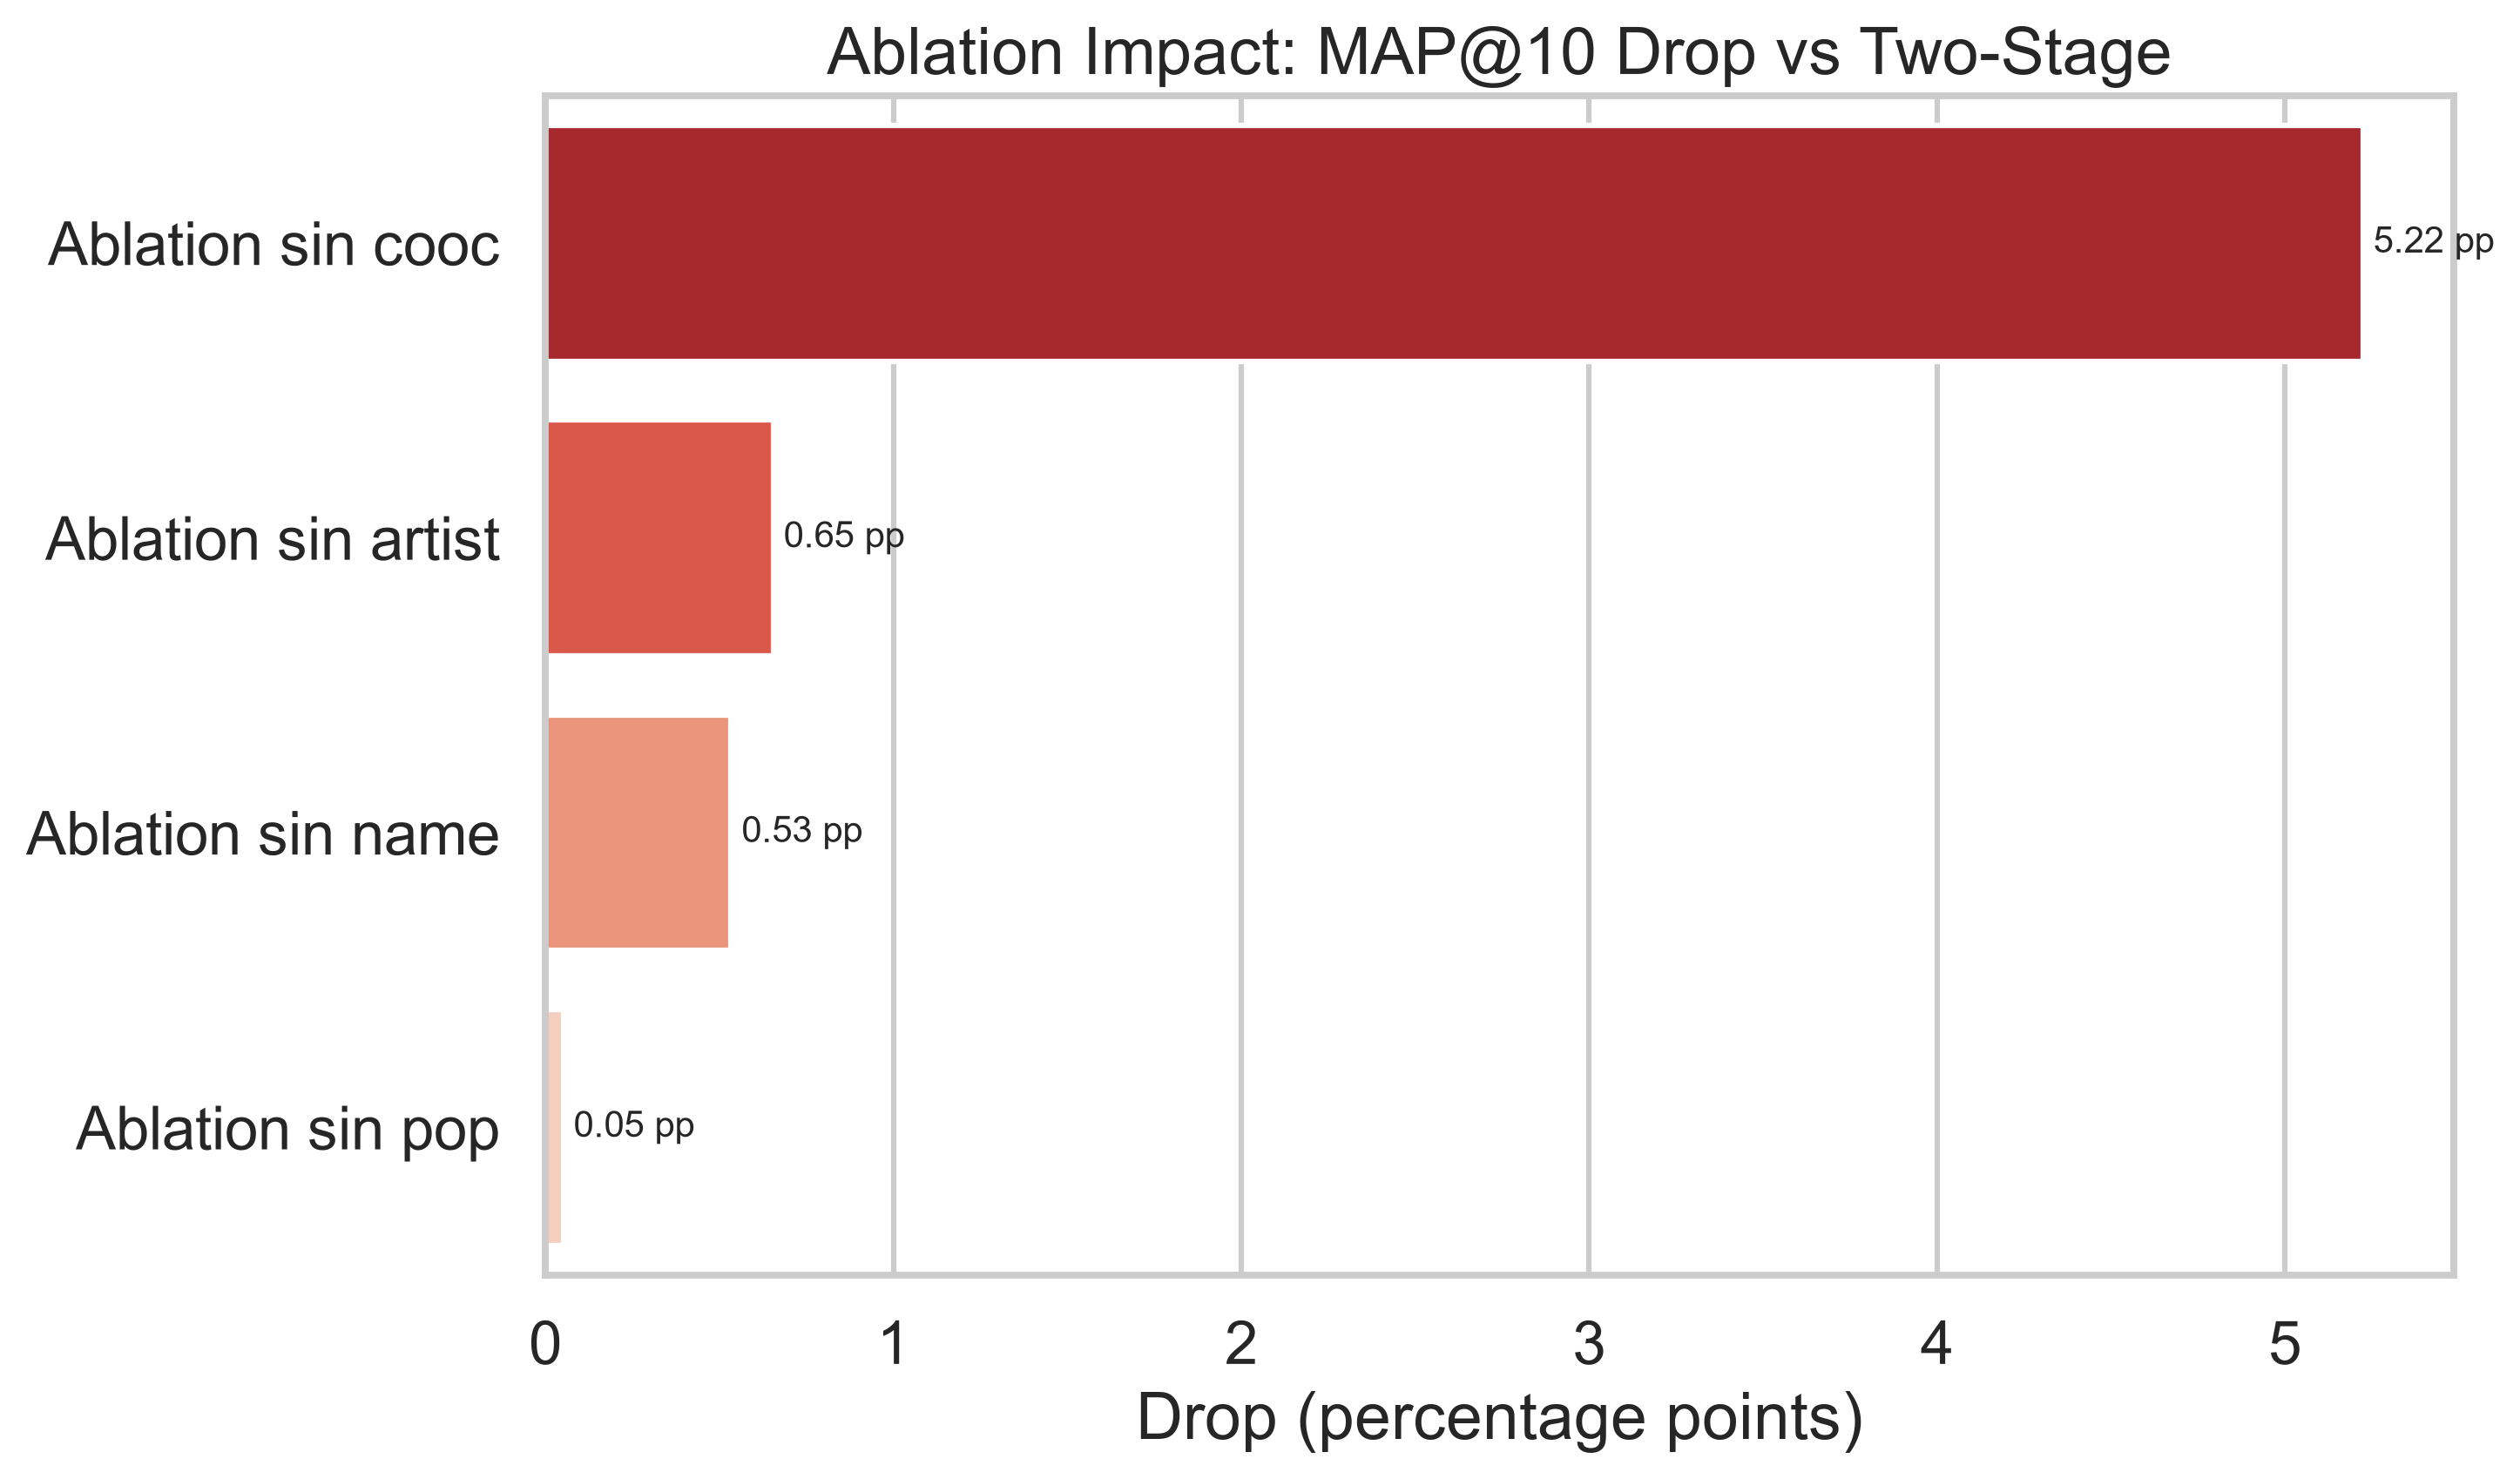
\includegraphics[width=0.98\linewidth]{figures/fig_ablation_map_drop.png}
\end{block}
\end{column}
\begin{column}{0.49\linewidth}
\begin{block}{Sensibilidad (20\%)}
\centering
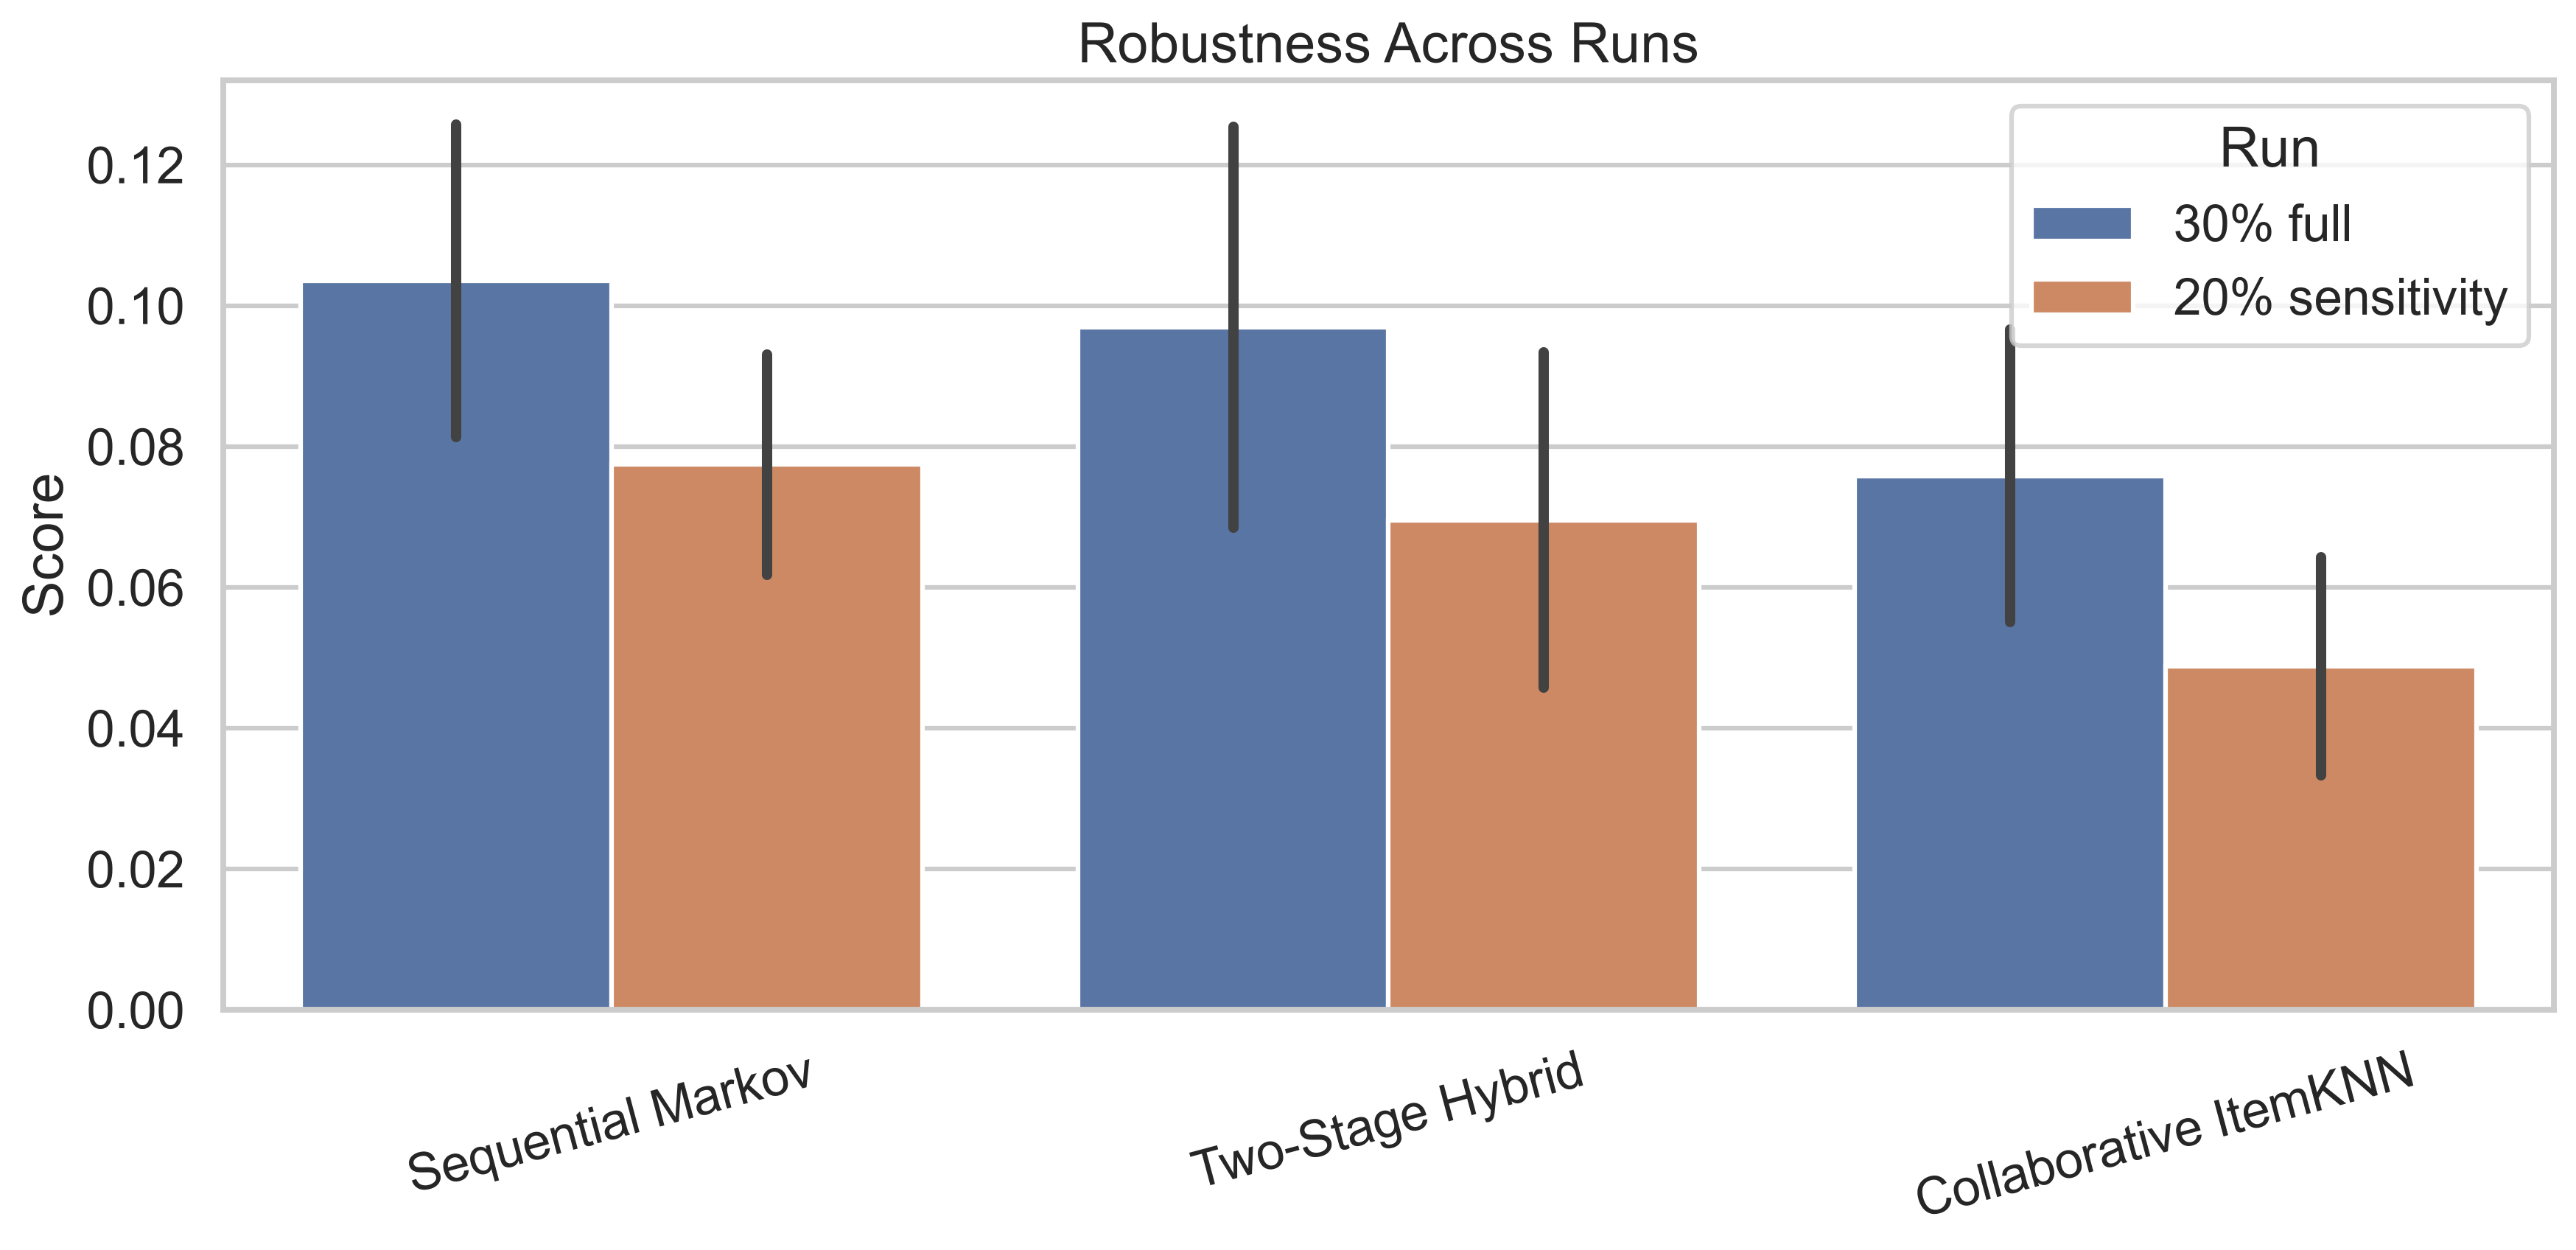
\includegraphics[width=0.98\linewidth]{figures/fig_sensitivity_comparison.png}
\end{block}
\end{column}
\end{columns}

\begin{block}{Beyond-accuracy}
\centering
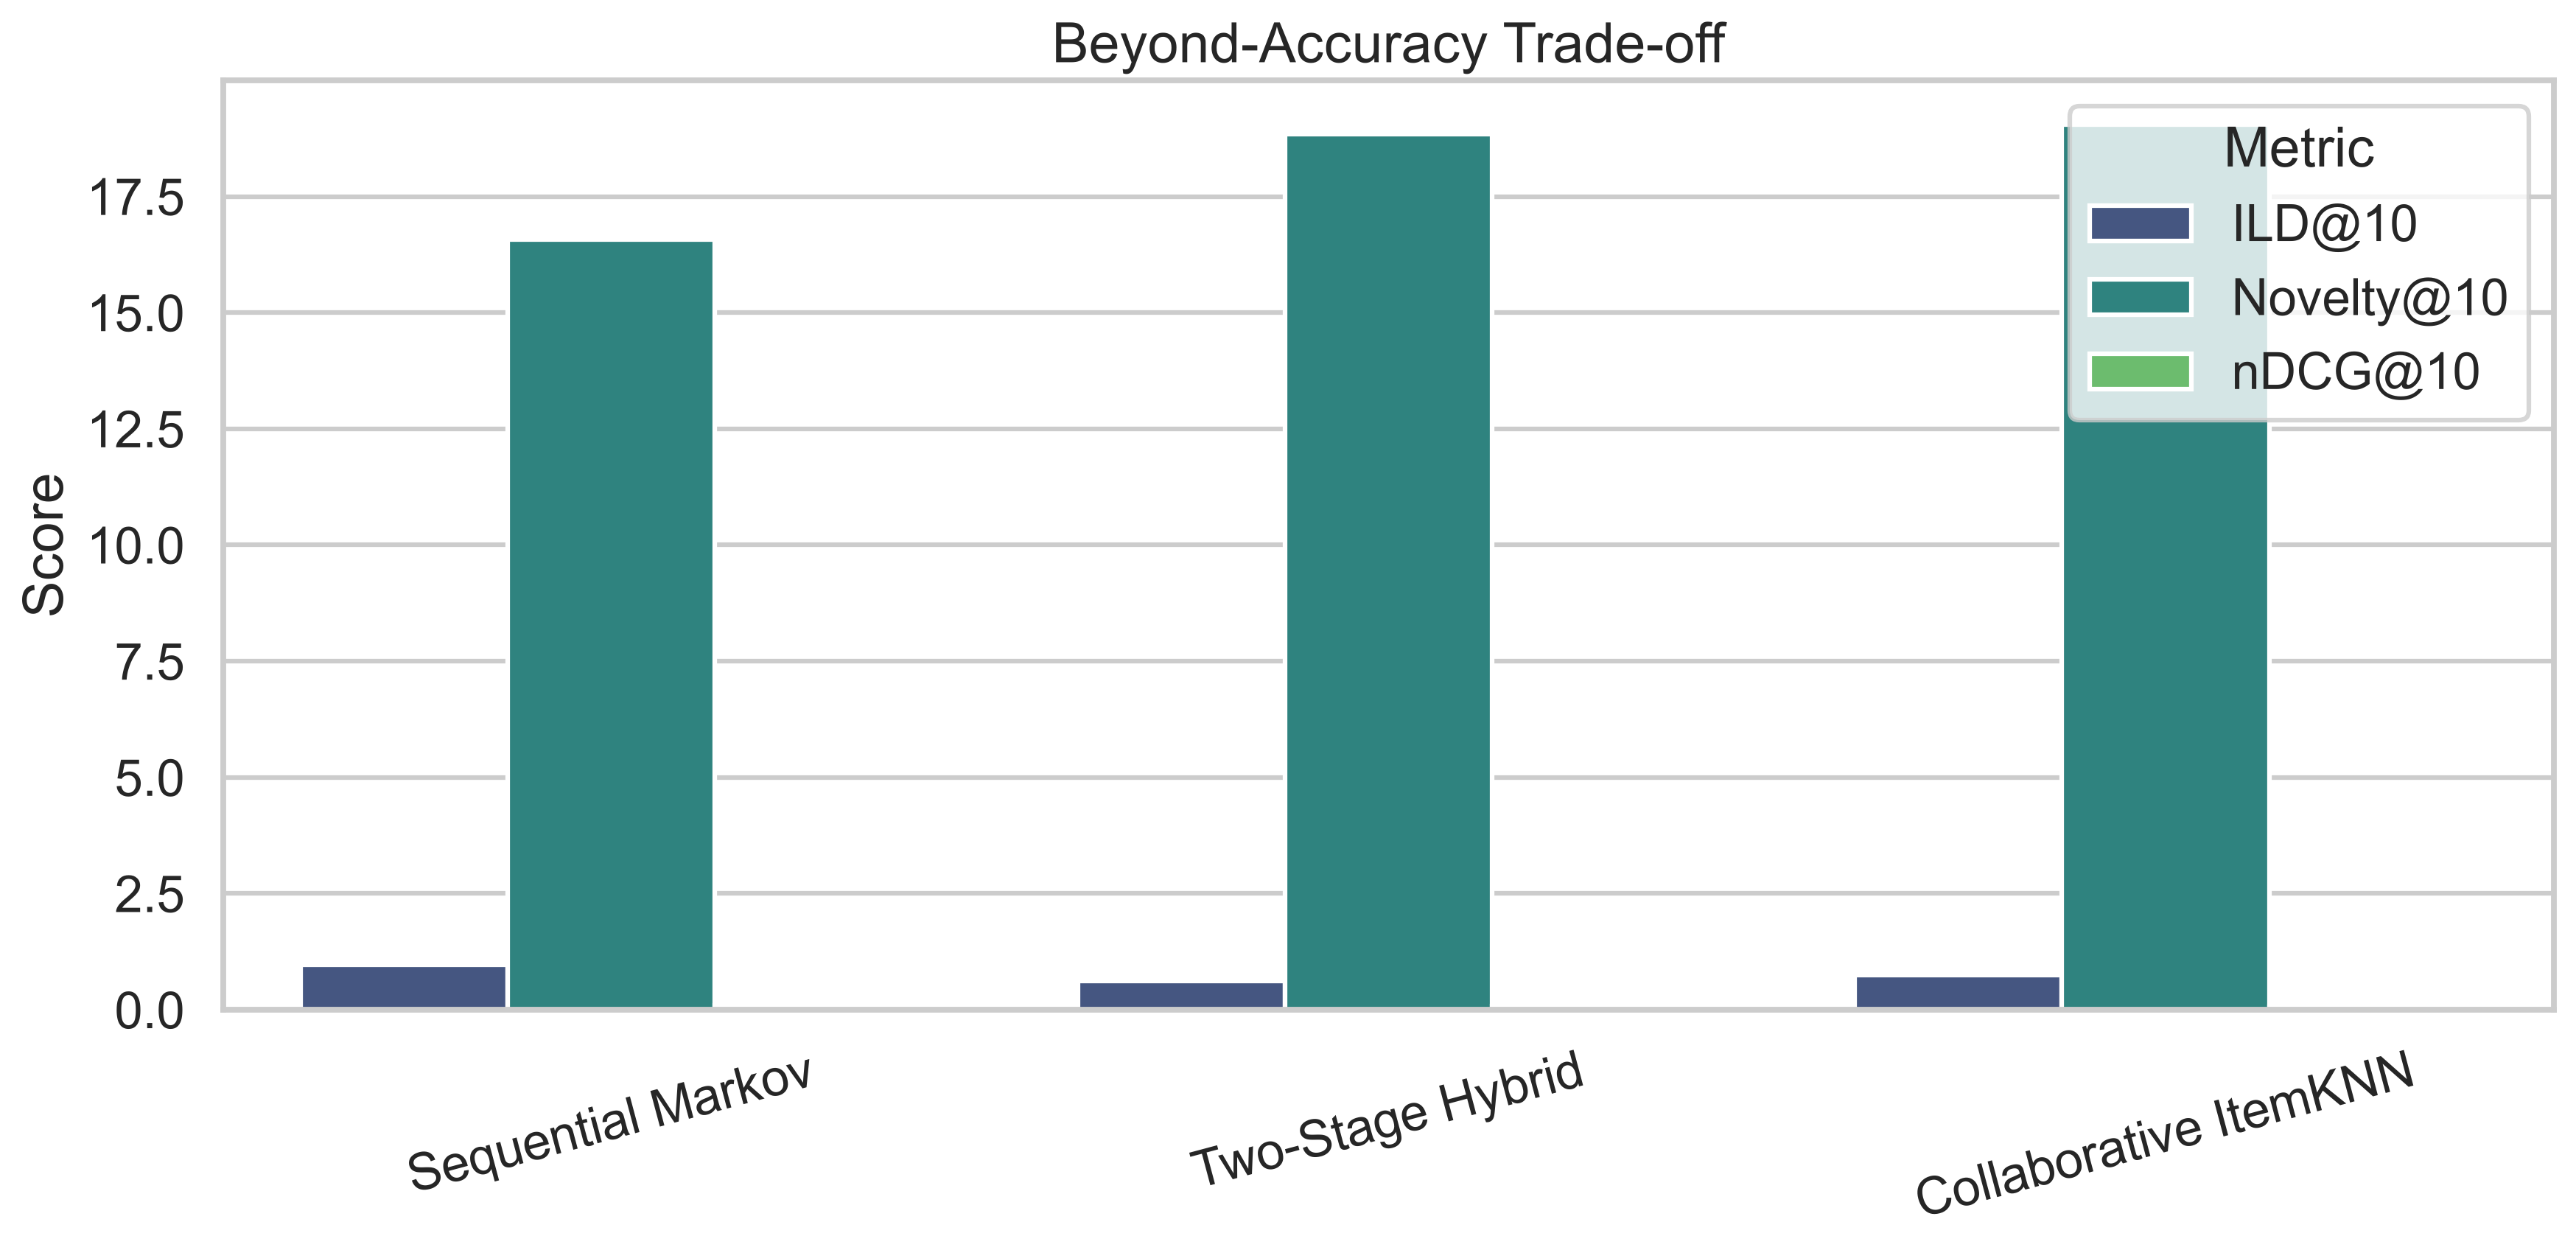
\includegraphics[width=0.98\linewidth]{figures/fig_beyond_accuracy.png}
\end{block}
\end{column}

\separatorcolumn

\begin{column}{\colwidth}
\begin{block}{Analisis por segmentos}
\centering
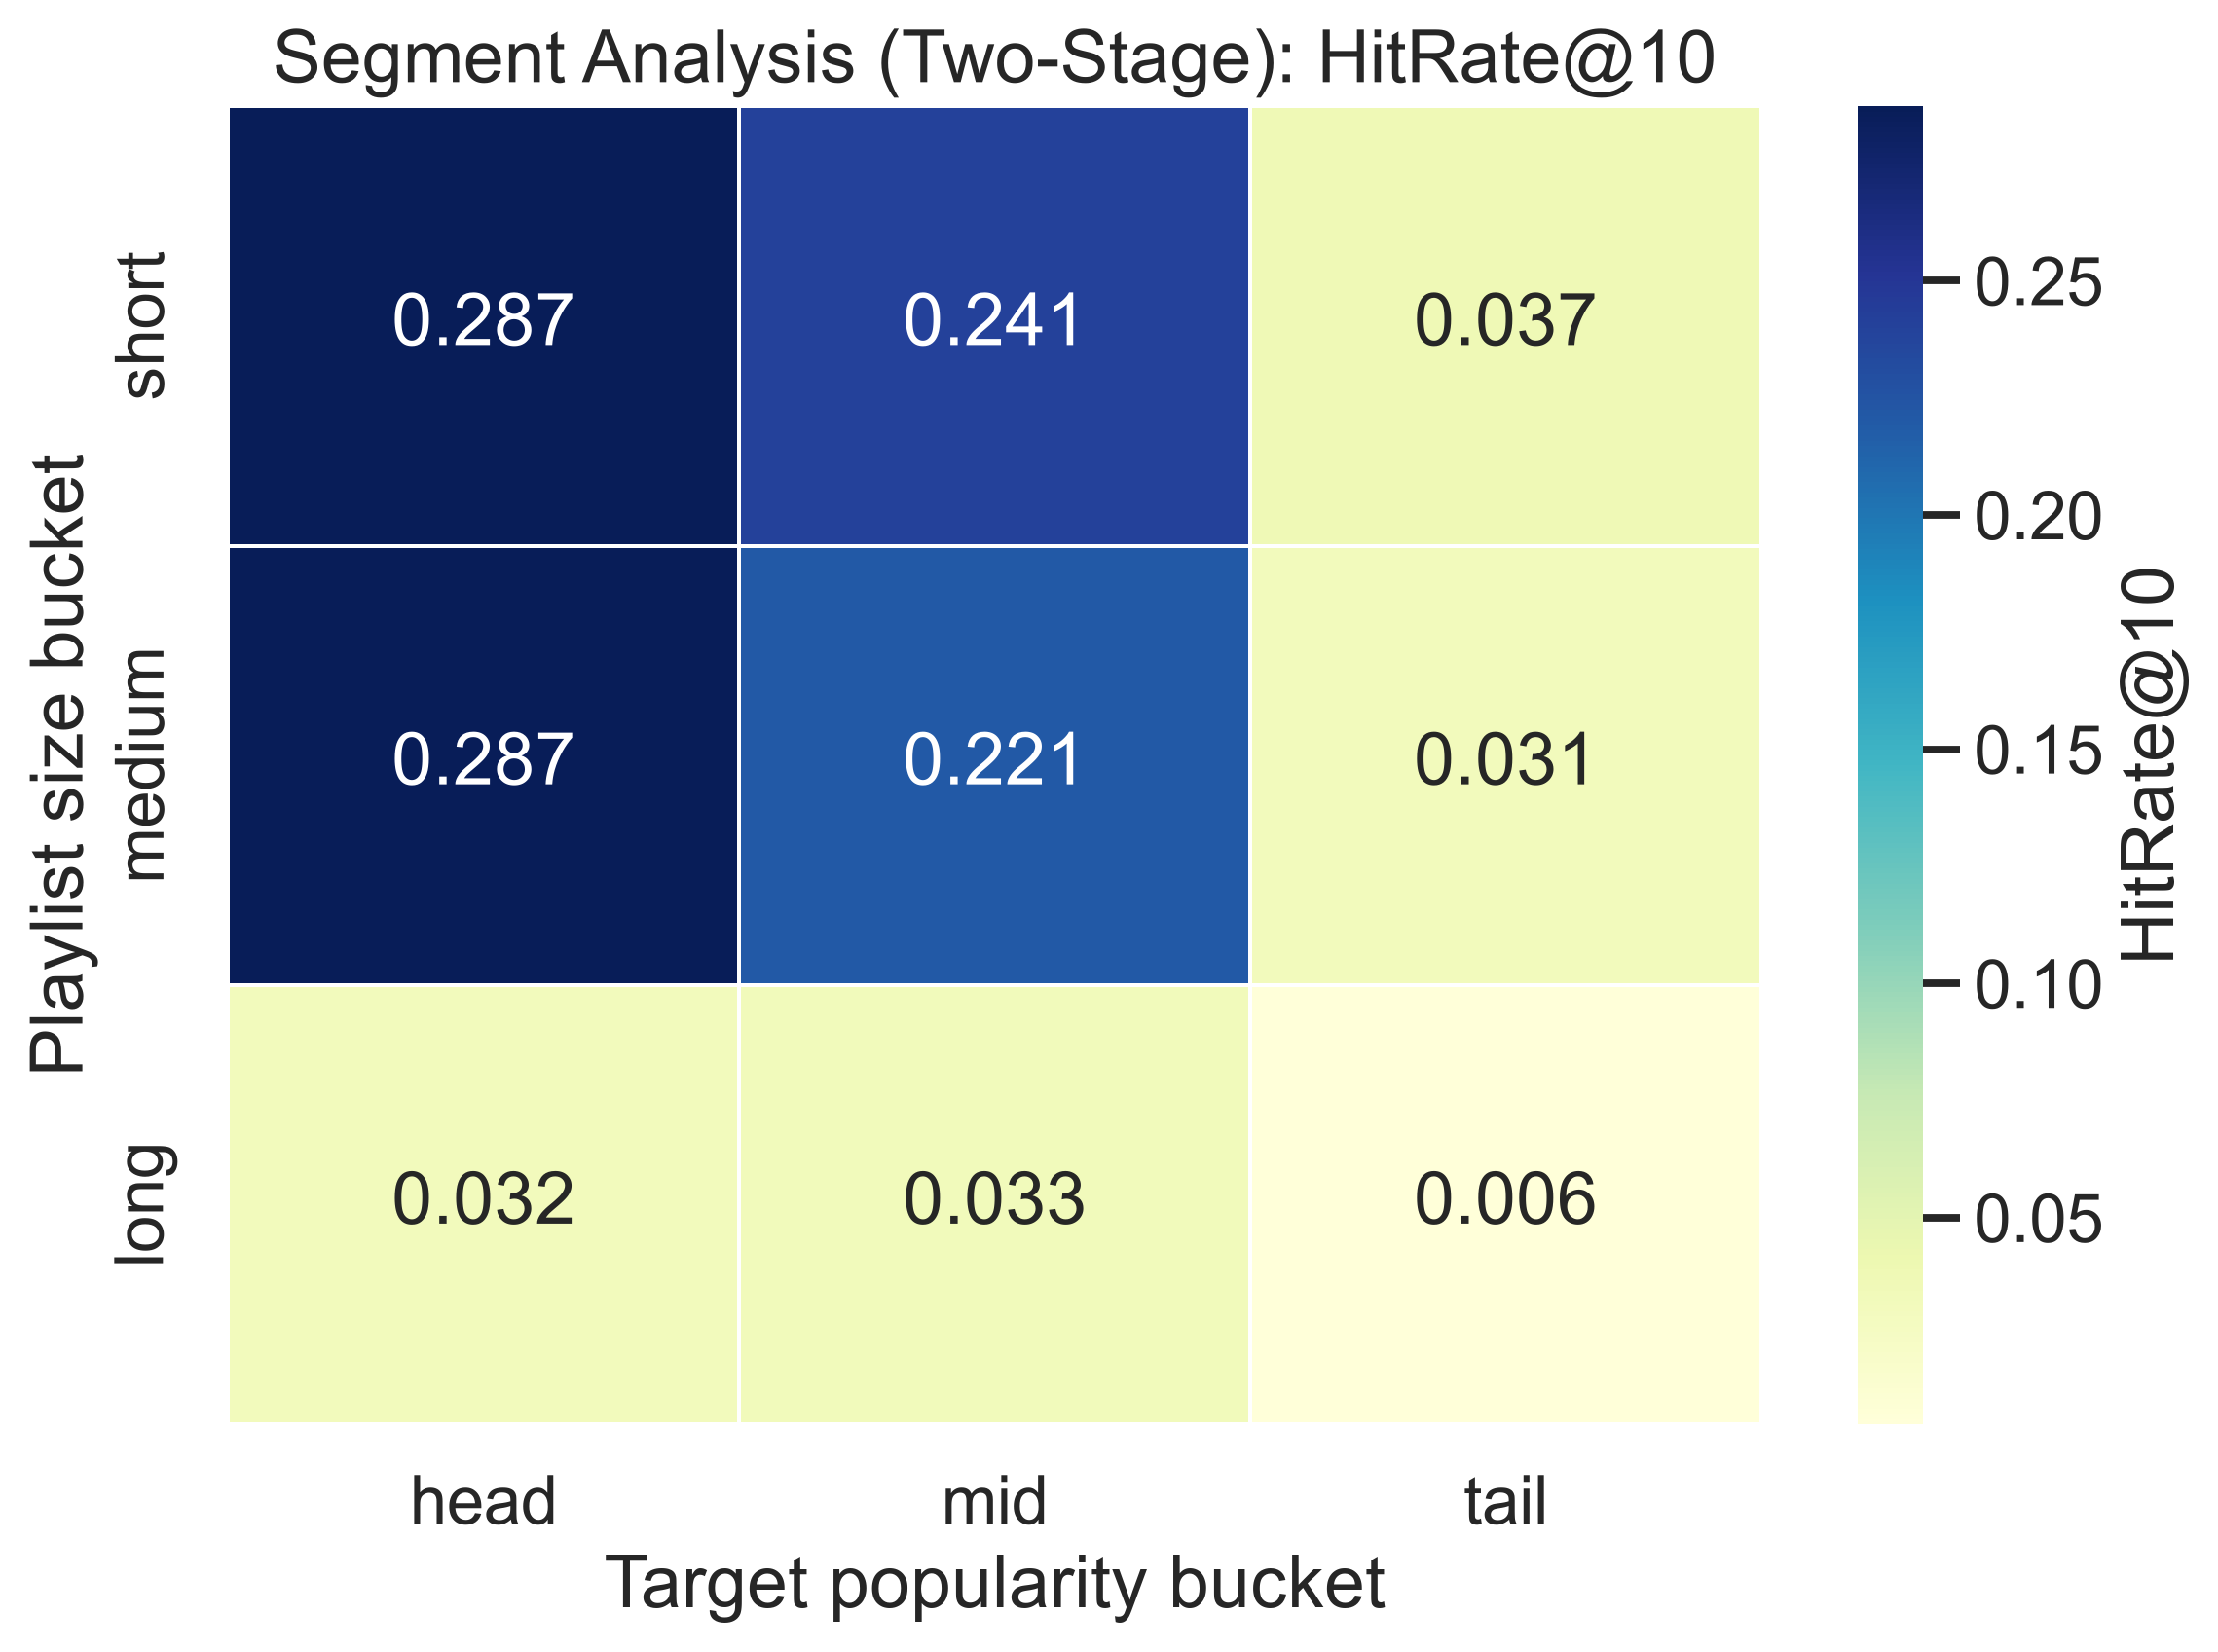
\includegraphics[width=0.98\linewidth]{figures/fig_segment_heatmap.png}
\end{block}

\begin{exampleblock}{Hallazgos}
\begin{itemize}
  \item Markov lidera en MAP/nDCG.
  \item Two-Stage mantiene HitRate competitivo y mejora cobertura de catalogo.
  \item La mayor caida aparece al remover cooc: senal dominante.
  \item El rendimiento cae en contexto largo + target tail.
\end{itemize}
\end{exampleblock}

\begin{alertblock}{Decision sobre LastFM}
LastFM se evaluo como enriquecimiento opcional, pero se excluyo del pipeline principal por latencia de API y reproducibilidad limitada a gran escala.
\end{alertblock}

\begin{block}{Conclusiones y trabajo futuro}
\begin{itemize}
  \item Two-Stage Hybrid es una base robusta y reproducible para APC.
  \item Se requiere evaluacion con baselines fuertes para comparacion justa.
  \item Futuro: reranking para cola larga y embeddings semanticos livianos.
\end{itemize}
\end{block}
\end{column}

\separatorcolumn
\end{columns}
\end{frame}
\end{document}
